\section{Speech Signal Processing}

\begin{frame}
\frametitle{Pre-emphasis}
\begin{itemize}
\item Pre-emphasis filter is essentially an \textbf{high-pass} filter.
\vspace{15pt}
\item Voiced speech naturally have an attenuation of $\sim$ 20 dB per decade due to physiological characteristics of the speech production system \cite{picone1993signal}.
\begin{itemize}
\item compensates this natural attenuation before spectral analysis.
\end{itemize}
\vspace{15pt}
\item Hearing is more sensitive to the components higher than 1 kHz.
\begin{itemize}
\item caters to human perception of sound
\end{itemize}
\end{itemize}
\end{frame}

%----------------------------------------------------------------------------------------
%	Subsection
%----------------------------------------------------------------------------------------

\begin{frame}
\frametitle{Framing \& Windowing}
\begin{itemize}
	\item speech signals are time-varying signals.
	\item the inertial motion of articulators
	\begin{itemize}
		\item speech can be considered statistically stationary in a short-time period ($\sim$ 30 ms) \cite{brandstein1995practical}.
		\item 30 ms $\longrightarrow$ 480 samples $\longrightarrow$ 512 (Radix-2 FFT)
	\end{itemize}
	\item Hamming window
	\begin{itemize}
		\item a compromise between \textbf{frequency resolution} and \textbf{spectral leakage}
	\end{itemize}
\end{itemize}
\end{frame}

%----------------------------------------------------------------------------------------
%	Subsection
%----------------------------------------------------------------------------------------

\begin{frame}
\frametitle{Threshold}
\begin{itemize}
\item distinguish informative frames from silent frames
\item two metrics: frame \textit{energy} and frame \textit{zero-crossing count}
\end{itemize}

\begin{figure}[H]
\centering
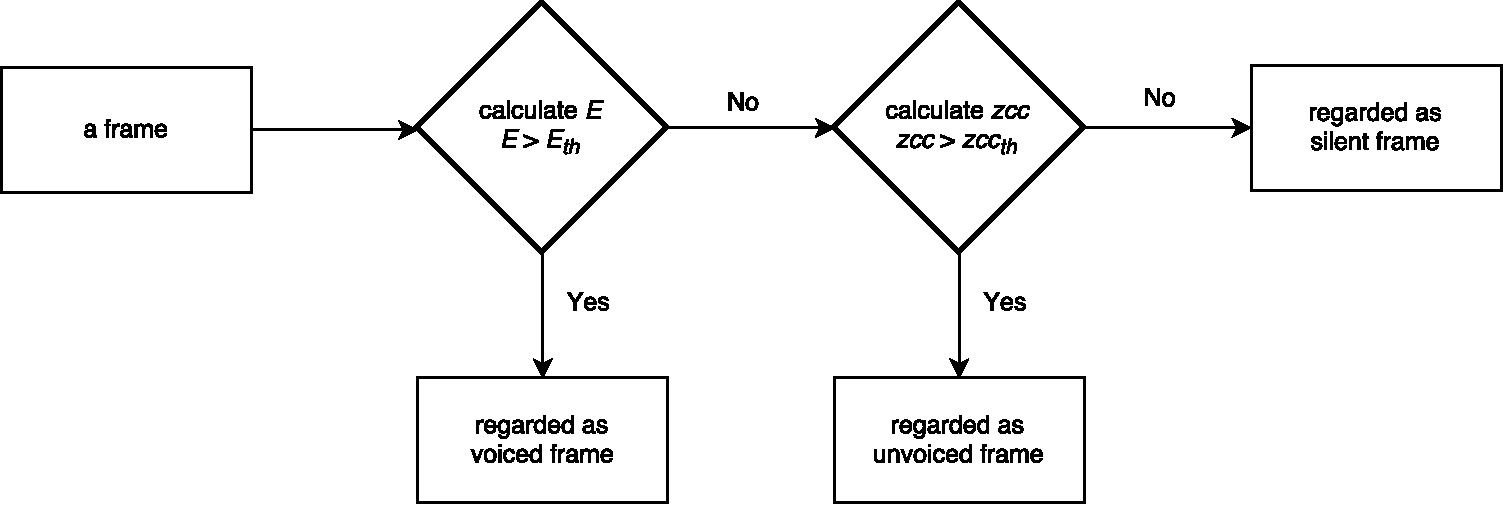
\includegraphics[width=\textwidth]{ang/threshold2}
\caption{decision-making strategy}
\end{figure}
\end{frame}

%----------------------------------------------------------------------------------------
%	Subsection
%----------------------------------------------------------------------------------------

\begin{frame}
\frametitle{Mel-frequency Cepstral Coefficients Extraction}
\begin{equation}
X[n] = \mathcal{F}^{-1} \left\{\log_{10} \left( |\mathcal{F}\{s[n]\}|^2 \right) \right\}
\end{equation}
\vspace{10pt}

The whole process to evaluate \textit{power cepstrum} can be divided into three procedures.
\begin{enumerate}
\item Compute the Discrete Fourier Transform $S_j[k]$ and corresponding power spectrum $\hat{S}_j[k]$ of a time-domain signal $s_j[n]$.
\item Take the logarithm of the power spectrum $\hat{S}_j[k]$.
\item Conduct inverse Fourier transform.
\end{enumerate}
\end{frame}

%--------------------------------------------
%--------------------------------------------

\begin{frame}
\frametitle{I. Power spectrum}

Discrete Fourier Transform
\begin{equation}
S_j[k] = \sum_{n=1}^{N} s_j[n] W_N^{(n-1) k} \quad k = 1, 2, \dots, N
\end{equation}
\begin{equation}
W_N = e^{\frac{- 2\pi i}{N}}
\end{equation}

Power Spectrum
\begin{equation}
\hat{S}_j[k] = |S_j[k]|^2 \quad k = 1, 2, \dots, \frac{N}{2} + 1
\end{equation}
\end{frame}

%--------------------------------------------
%--------------------------------------------

\begin{frame}
\frametitle{II. Bank Filtering}
\begin{itemize}
	\item Human hearing responds to the entire critical band instead of individual frequencies in this band.
	\item $M = 20$ banks
\end{itemize}

\begin{figure}[H]
\centering
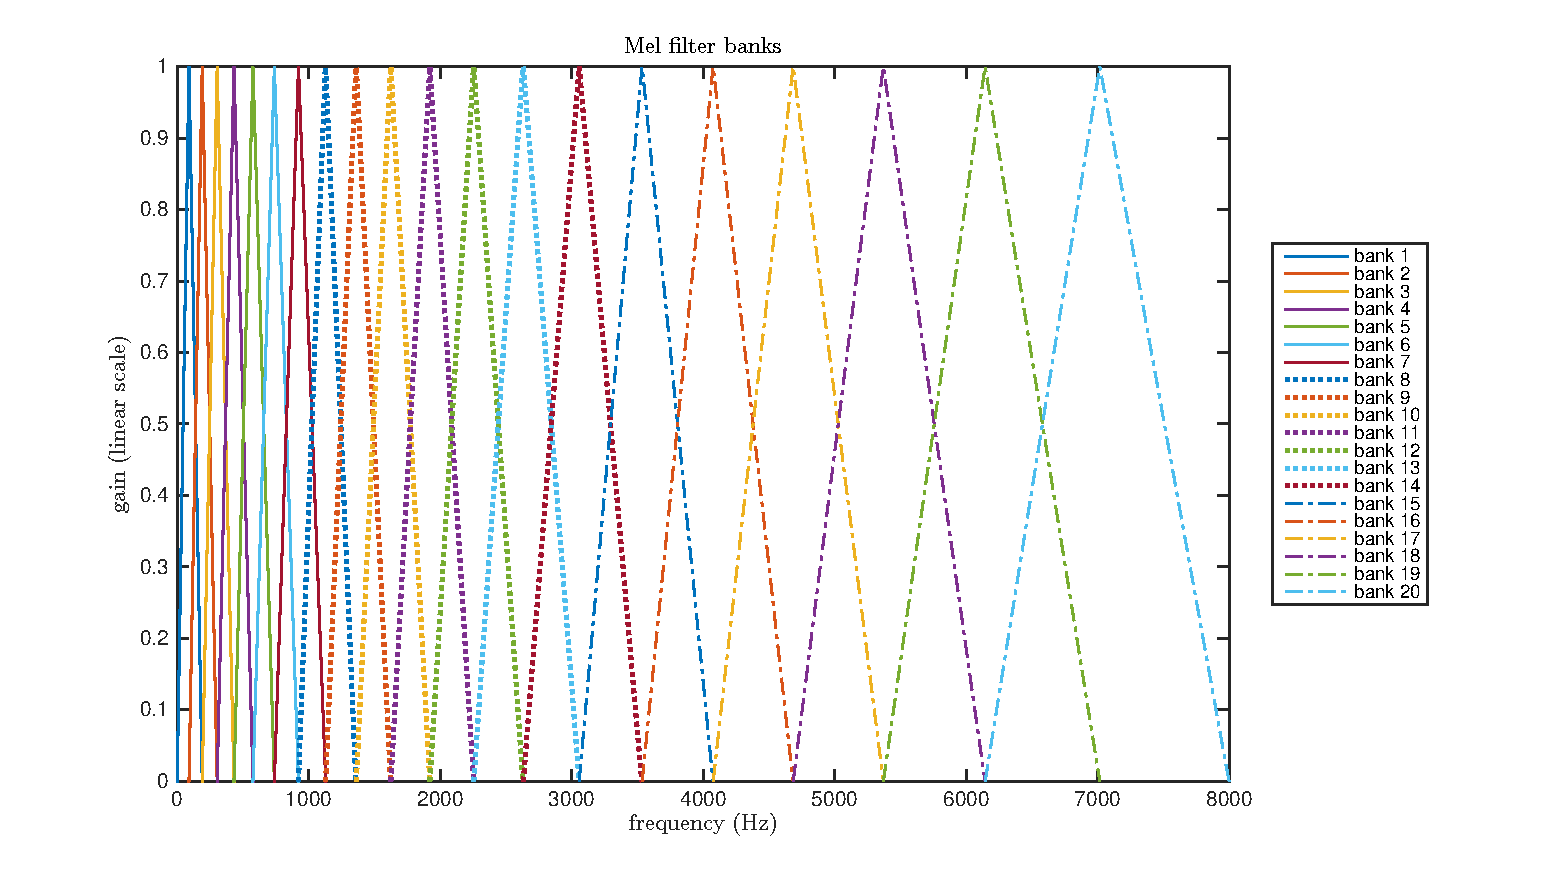
\includegraphics[width=0.9\textwidth, trim={0 0.6cm 0 0.6cm}, clip]{ang/mel_triangle}
\end{figure}
\end{frame}

%--------------------------------------------

\begin{frame}
\begin{enumerate}
\item Each power spectrum data point (\textcolor{gold_matlab}{gold circle $\circ$}) is multiplied by the corresponding gain (\textcolor{orange_matlab}{orange asterisk $*$}).
\item \textcolor{orange_matlab}{Orange crosses $\times$} represent the scaled power spectrum.
\item Total power within bank $m=9$ is the sum of all scaled power data points.
\end{enumerate}

\begin{figure}[H]
\centering
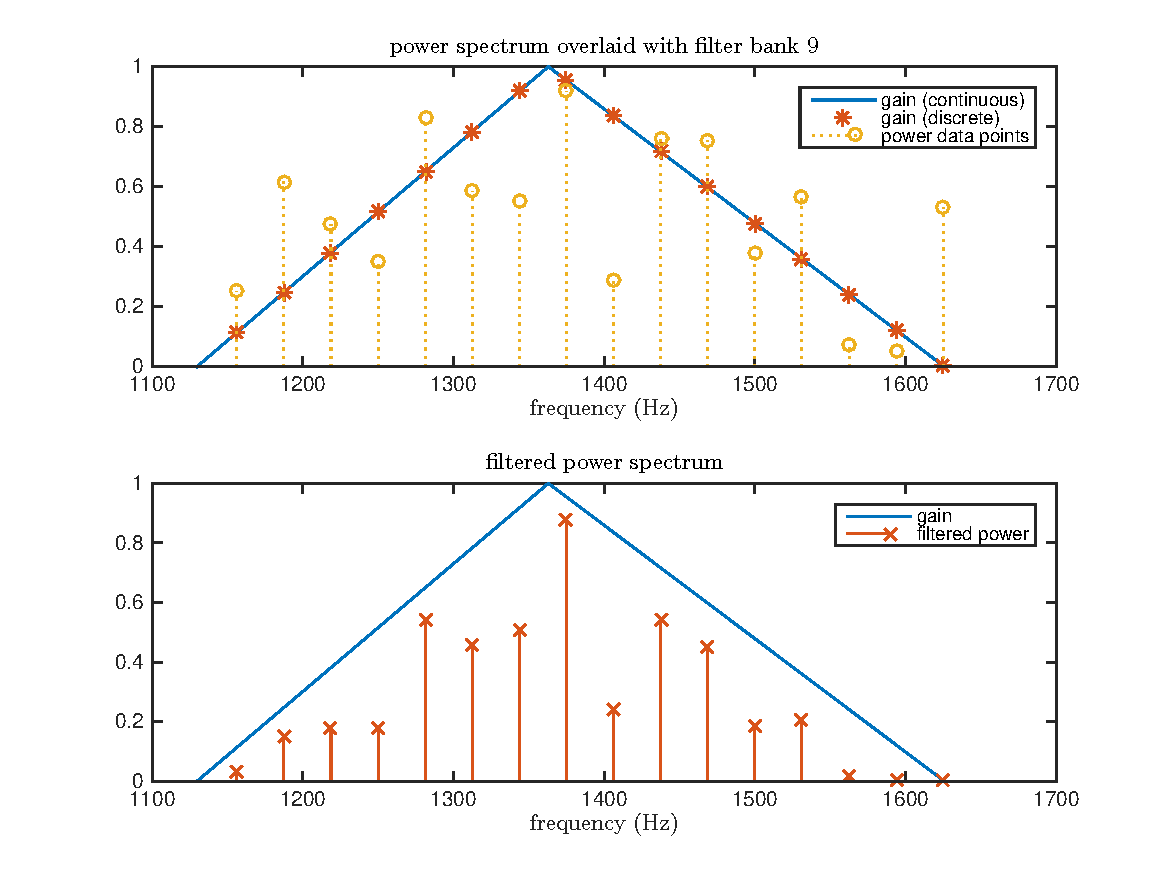
\includegraphics[width=3in, trim={0 0.6cm 0 0.6cm}, clip]{ang/bank_filter_demostration}
\end{figure}
\end{frame}

%--------------------------------------------
%--------------------------------------------

\begin{frame}
\frametitle{III. Log Scaling}
\begin{equation}
\hat{X}_j[m] = \log_{10}(X_j[m]) \quad m = 1, 2, \dots, M
\end{equation}

\begin{enumerate}
\item Log scaling makes the system more resilient to both very quiet and very loud sound.
\item Log scale in dB imitates human nonlinear perception to loudness \cite{farin2008mathematical}.
\item Without taking logarithm, recognition accuracy is severely reduced \cite{tan2008automatic}.
\end{enumerate}
\end{frame}

%--------------------------------------------
%--------------------------------------------

\begin{frame}
\frametitle{IV. Discrete Cosine Transform}
IDFT is replaced by Discrete Cosine Transform due to the symmetric and real characteristic of log power spectrum $\hat{X}_j[m]$ \cite{picone1993signal, iser2008bandwidth}.

\begin{itemize}
	\item The order of DCT ($F$) determines the amount of MFCCs. \cite{tan2008automatic}
	\begin{itemize}
		\item Higher-order coefficients incorporate excitation information.
		\item Lower-order coefficients indicate the slowly varying vocal tract.
	\end{itemize}
	\item European Telecommunications Standards Institute adopts $F = 13$ in their speech recognition standard \cite{etsi2001202}.
	\item We also condense the $M$-point sequence $\hat{X}_j[m]$ into a shorter $F$-point sequence $\hat{C}_j[n]$. The choice of $F$ will be further discussed in \textit{Design \& Performance} section.
\end{itemize}
\end{frame}
